%%%%%%%%%%%%%%%%%%%%%%%%%%%%%%%%%%%%%%%%%%%%%%%%%%%%%%%%%%%%%%%%%%%%%%%%
%                                                                      %
%     File: Thesis_Results.tex                                         %
%     Tex Master: Thesis.tex                                           %
%                                                                      %
%     Author: Carlos A. Rodrigues                                      %
%     Last modified : 21 Jan 2011                                      %
%                                                                      %
%%%%%%%%%%%%%%%%%%%%%%%%%%%%%%%%%%%%%%%%%%%%%%%%%%%%%%%%%%%%%%%%%%%%%%%%

%\usepackage{caption} 
\captionsetup[table]{skip=-3pt}


\chapter{Estrutura do compilador}
\label{chapter:estrutura_do_compilador}

Um compilador converte um código numa linguagem definida (como Java, C, C++, etc) para uma linguagem máquina. Quando se constrói um compilador, é necessário
 construir a conversão da linguagem para um {\it assembly} compativel com a máquina onde se está a trabalhar, o que dava um compilador diferente para cada linguagem e para
 cada máquina. Tal não acontece graças a uma representação intermediária universal, que divide o processo de compilação entre dois passos: o 
 {\it front end} e o {\it back end}. Tal como no GCC, o compilador do Versat está dividido em duas partes: o {\it front end} e o {\it back end}.  Em muitos compiladores existe um passo intermédio entre a representação intermédia e o {\it back end} que é o passo de optimização. 
 Devido à simplicidade dos programas em Versat, não foi implementado o passo de optimização.   
 
No {\it front end} é realizada a conversão para a representação intermédia. O {\it front end} está dividido em 3 fases:
\begin{itemize}
  \item {\it Scanning};
  \item {\it Parsing};
  \item Análise semantica. Tradução da árvore de sintaxe abstracta para a estrutura de dados intermédia.
\end{itemize}

O {\it scanning} lê os caracteres e converte-os em {\it tokens}. Um {\it token} é uma sequência de símbolos detectada durante a análise lexical. 

Depois da análise lexical, é feita a análise sintáctica. A análise sintáctica é a construção da árvore de {\it parse}, analisando uma sequência de {\it tokens} 
e arranjar alguma regra gramatical compatível com a sequência recebida. Caso não seja detectada alguma regra gramatical existente, o compilador informa o utilizador que existe um erro.

Depois de concluída a análise sintáctica, é preenchida a estrutura de dados intermédia com o objectivo de através dela produzir o {\it assembly}.
O {\it back end} é a parte responsável por ler a estrutura intermédia e gerar o respectivo {\it assembly}. O {\it back end} está dividido em 3 fases:

\begin{itemize}
  \item Leitura da estrutura intermédia e geração do respectivo {\it assembly};
  \item Optimização do {\it assembly};
  \item Geração do código máquina através do {\it assembly}.
\end{itemize}

\textcolor{red}{discutir com o professor sobre a junção do assembler com o compilador e melhoramento do assembler!!!!!!!!!!}
O compilador não produz o código máquina. Para a produção do código máquina, é necessário usar o {\it assembler} do Versat que está à parte do compilador. 
O compilador do Versat não faz optimizações de {\it assembly}.

\section{Front end}
\label{chapter:front end}

No compilador do Versat, tal como nos compiladores convencionais, a estrutura de dados intermédia é construída através de ferramentas que efectuam as análises sintáctica e lexical.
As ferramentas usadas para a construção do {\it front end} são o Flex (analisador lexical) e o Bison (analisador sintáctico).

O Flex é o responsável pela análise lexical do compilador. O Flex lê os caracteres e converte-os em {\it tokens}, também é responsável por:

\begin{itemize}
  \item Reconhecer palavras chave na linguagem;
  \item Ignorar espaços em branco e comentários;
  \item Reconhecer números e {\it bits}.
\end{itemize}

%Considera-se a instrução em C++ do Versat:
%\begin{lstlisting} 
 %     aluLite2.setOper("+");      
%\end{lstlisting}  

%O Flex detecta os {\it tokens} ``aluLite2''  '.'  ``setOper''  '('  '  '+' ' ')'  ';'. %, ``.'', ``setOper'', ``('' ``"'' ``+'' ``"'' ``)'' ``;''. 

Depois de detectados os {\it tokens}, é feita a análise sintáctica. A análise sintáctica é realizada pelo programa Bison.
O Bison é um gerador de {\it parse}. Recebe uma série de {\it tokens} e procura uma regra gramatical que seja compativel com a sequência que recebeu. Também
avisa caso exista alguma ambiguidade gramatical e caso não seja detectada nenhuma regra gramatical compativel com a sequência recebida, activa a directoria
yyerror e informa que houve um erro.

Considera-se um ciclo while em C++ do Versat.

\begin{lstlisting} 
      while(R1<10)      
\end{lstlisting}  

O bison recebe os vários {\it tokens} e procura uma regra gramatical existente. 


A árvore do {\it parse} gerada pelo bison está representada na figura~\ref{fig:arvore while}.

Onde:

\begin{itemize}
  \item whl\_units é o ramo que espera receber o {\it token} while;
  \item reg\_units é o ramo que recebe o registo usado no primeiro operando;
  \item sif\_operators tem as condições sentenciais;
  \item reg\_const representa as constantes.
\end{itemize}


\pagebreak

\begin{figure}[!htb]
  \centering
  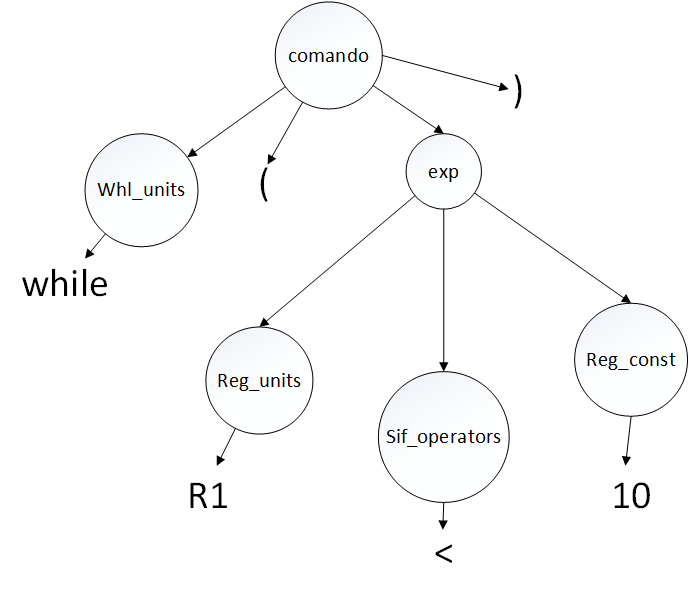
\includegraphics[height=100mm, width=130mm]{Figures/parse_do_ciclo_while.png}
  \caption[Árvore gerada do ciclo {\it while}.]{Árvore gerada do ciclo {\it while}.}  
  \label{fig:arvore while}
\end{figure}



É necessário existir ramos com o objectivo de guardar os dados recebidos na estrutura de dados intermédia.


%\textcolor{red}{Ainda não suporta a ideia de R1++}

Considera-se uma instrução do Data Engine.

\begin{lstlisting} 
     mem0.portB.setStart(2);   
\end{lstlisting}  

A árvore do {\it parse} gerada pelo bison está representada na figura~\ref{fig:arvore mem0}.

Onde:

\begin{itemize}
  \item Mem units é a memória em causa;
  \item Ports é o porto de memória em causa;
  \item Mem\_methods é o método em causa;
  \item Mem units é a memória em causa;
  \item Expressions2 e expression são os ramos que geram a expressão da árvore.
\end{itemize}



\begin{figure}[!htb]
  \centering
  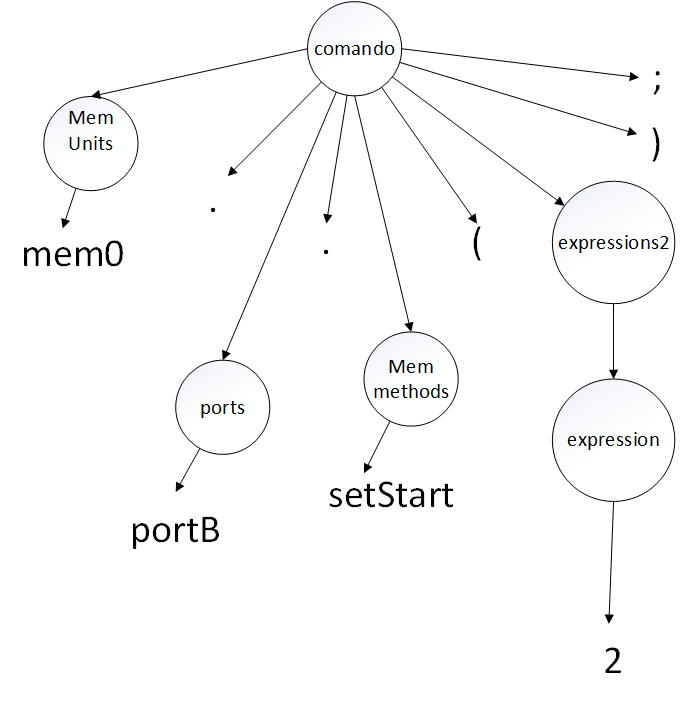
\includegraphics[height=110mm, width=120mm]{Figures/parse_do_mem0.png}
  \caption[Árvore da instrução de configuração do gerador de endereços.]{Árvore da instrução de configuração do gerador de endereços.}  
  \label{fig:arvore mem0}
\end{figure}

\pagebreak

O estado de erro não é representado nos esquemas das figuras~\ref{fig:arvore exp},~\ref{fig:arvore mem0} e~\ref{fig:arvore while}, mas quando não se encontra nenhuma sequência compativel
com a sequência que se recebeu vai para o estado de erro. 

\textcolor{red}{(perguntar isto ao professor)}

Considera-se uma expressão em C++ do Versat.

\begin{lstlisting} 
     R5 = R4+R3+(2-R6);   
\end{lstlisting}  

A árvore do {\it parse} da expressão está representada na figura~\ref{fig:arvore exp}.

Onde:

\begin{itemize}
  \item Reg\_target é o registo onde o resultado vai ser guardado;
  \item Expressions é o ramo responsável por guardar os dados da expressão na estrutura de dados intermédia.
\end{itemize}

\begin{figure}[!htb]
  \centering
  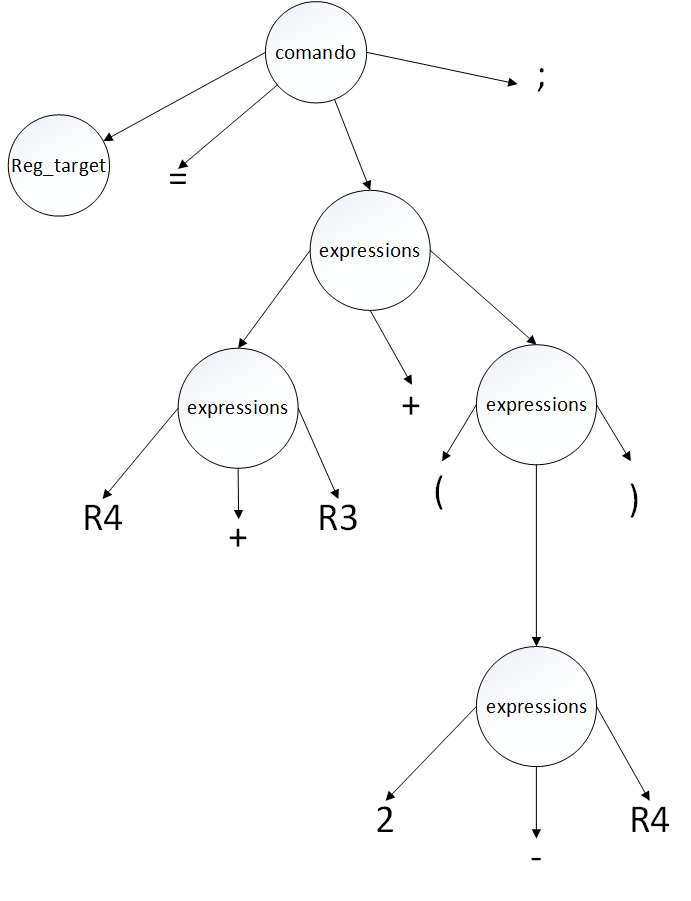
\includegraphics[height=130mm, width=130mm]{Figures/parse_da_expressao.png}
  \caption[Árvore gerada do ciclo {\it while}.]{Árvore gerada do ciclo {\it while}.}  
  \label{fig:arvore exp}
\end{figure}

\pagebreak


Para processar as expressões, é usada uma estrutura de dados em forma de árvore binária, associada ao comando.

\section{Back end}
\label{chapter:back end}

Depois de concluido o {\it parse}, a estrutura de dados é preenchida. A estrutura de dados é uma lista de tipo comando, que tem 
todas as estruturas necessárias para gerar o {\it assembly}. Esta estrutura de dados é constituída pelo seginte pseudo-código:

\textcolor{red}{Tirar isto e meter pseudo-código!!!!!!!!!!!!!!!!!!!!!!!}

\begin{lstlisting}
		tipo de comando;
		unidade;
		porto;
		método;
		NODE *árvore de registos;
		NODE2 *árvore de expressões;

		operador;
		operando1;
		operando2;
		tipo do operador1;
		tipo do operador2;
		
		etiqueta;
		
		GenFU _genFU;
		GenMem _genMem;
		ctrlReg _ctrlReg;
		controller _controller;
\end{lstlisting}

Existem outros atributos auxiliares usados no {\it back end}, porém não estão representados no pseudo-código.

O apontador de tipo NODE é a base da árvore que gera as expressões. É nesta estrutura que se guarda as expressões de registos e se gera o {\it assembly} pela ordem correcta.
O tipo NODE2 é responsável pela geração das expressões de memória. 

As classes \_genFU, \_genMem, \_ctrlReg e \_controller são responsáveis pela geração de {\it assembly} das unidades funcionais, pelas instruções de inicialização, arranque, espera e pelas instruções ligadas ao controlador como por exemplo, as expressões.

\textcolor{red}{Fazer um diagrama UML da estrutura de dados  }

Considera-se um ciclo for em C++ do Versat.

\begin{lstlisting}
 int main() {

	for(R1=0;R1<10;R1=R1+1) {
		R5 = R5+R1; }
		
return 0;     }
\end{lstlisting}

O respectivo código {\it assembly} gerado é:

\begin{lstlisting}
 
	ldi 0
	wrw R1
forDirectStatment0	rdw R1
	addi -10
	wrw RB
	ldi 0
	ldih 0x8000
	and RB
	beqi forStatment0
	nop 
	nop 
	rdw R5
	add R1
	wrw R5
	rdw R1
	addi 1
	wrw R1
	ldi 0
	beqi forDirectStatment0
	nop 
forStatment0 nop
	ldi 0
	beqi 0
	nop

\end{lstlisting}

Estão representadas algumas das etiquetas que o utilizador não pode usar no programa, por estarem relacionadas com a geração dos ciclos (consultar tabela~\ref{tab:labels}).

Considera-se uma expressão em Versat.

\begin{lstlisting} 
     R5 = R4+R3+(2-R6);   
\end{lstlisting} 

A respectiva árvore de sintaxe abstracta é dada na figura~\ref{fig:arvore asa}.

\begin{figure}[!htb]
  \centering
  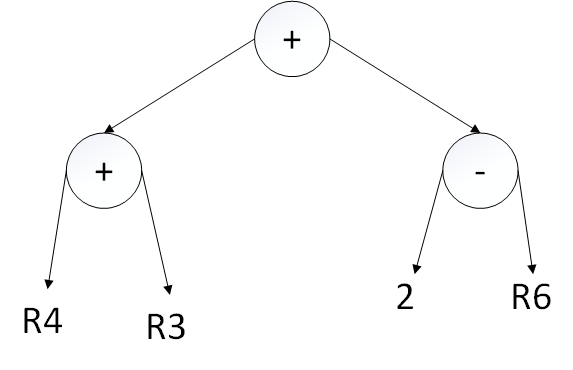
\includegraphics[height=70mm, width=90mm]{Figures/abstract_syntax_tree.png}
  \caption[Árvore de sintaxe abstracta.]{Árvore de sintaxe abstracta.}  
  \label{fig:arvore asa}
\end{figure}

A árvore é contruída no {\it front end}, enquanto no {\it back end} é realizada a leitura da estrutura de dados com o objectivo de gerar o respectivo {\it assembly}.

%\textcolor{red}{meter referencia da tabela}

\chapter{Variáveis e objectos pré-definidos}
\label{section:Linguagem definida}


É conveniente referir que optou-se por uma abordagem baseada em C++ para a linguagem do compilador. Esta decisão está directamente atribuída ao
facto de esta linguagem ser conhecida, o que facilita o trabalho de um programador, não necessitando de um processo de aprendizagem. Entretanto,
é convenente referir que o Versat não tem uma {\it stack} própria, sendo impossível criar funções em C++. Assim, neste processo de
programação não estão envolvidas funções.

No Versat trabalha-se com objectos e variáveis. Como os recursos são limitados, tanto as variáveis como os objectos já estão pré-definidos.


\section{Objectos e variáveis existentes}
\label{section:objectos existentes}

Os objectos e variáveis existentes no Versat encontram-se na tabela~\ref{tab:objvarex}.

\begin{table}[h!]
    \caption[Objectos e variáveis existentes.]{Objectos e variáveis existentes.}
  \begin{center}
    \begin{tabular}{|l|l|L{7cm}|}
      \hline
       Objecto/Variável & Número/letra da unidade funcional & Descrição  \\
      \hline \hline
     % \multirow{10}{*}{Wishbone} & wb\_clk\_i & input & Clock, Recebido pelo Wishbone. \\
      \cline{1-3}
      mem  & 0-3 & Memórias existentes no C++ do Versat.  \\
      \cline{1-3}
       alu & 0-1 & Alus existentes no C++ do Versat. \\
       \cline{1-3}
       aluLite & 0-3 & AluLites existentes no C++ do Versat.  \\
       \cline{1-3}
       mult & 0-3 & Multiplicadores existentes no C++ do Versat. \\
       \cline{1-3}
       de\_ctrl\_reg & - & Representante dos registos de controlo e de estado. \\
       \cline{1-3}
       port & A-B & Portos de memória existentes no Versat. Cada memória tem dois portos com configurações independentes.  \\
       \cline{1-3}
       Bs & 0 & {\it Barrel shifters} existentes no C++ do Versat.  \\
       \cline{1-3}
       R & 1-14 & Registos permitidos para uso como variáveis no C++ do Versat. Também existem os registos R0 e R15, mas estes são usados internamente pelo {\it hardware} do Versat. \\
       \cline{1-3}
       RB & - & Registo B. Apesar deste registo ser utilizado como apontador, o uso dele como variável é permitido.  \\
       \cline{1-3}
       mem & 0-3/A-B & Variáveis das expressões de memória. Nas expressões de memória, as memórias são tratadas como variáveis.  \\
       
       
      \hline
    \end{tabular}
  \end{center}
  \label{tab:objvarex}
\end{table}

Visto que cada memória tem dois portos com configurações independentes, os portos das memórias são tratados como objectos. 
É possível usar o registo RB como variável, mas este é usado internamente pelo compilador para cálculos auxiliares. 
O objecto de\_ctrl\_reg representa os registos de controlo e de estado, embora estes apresentem-se em separado. Esta abordagem tem o intuito
de facilitar o trabalho do programador.

\textcolor{red}{É preciso proibir o uso do RB!!!!!!!!!!!!!!!!}


\pagebreak

\section{int main}
\label{section:int main}


Tal como em C++ regular, os programas em C++ do Versat começam na função {\it main}. Não são suportadas as variáveis de argc e argv.

Um exemplo do inicio de uma função em C++ do Versat é dado da seguinte forma:

\begin{lstlisting}
 int main() {
	R4=5;
	return 0;  }
\end{lstlisting}

Refere-se que as directivas de pré-processador, tais como \#define e \#include, não são suportadas.


\textcolor{red}{Tirar o suporte do bison ao argc e ao argv}


\section{Métodos dos registos de controlo e de estado}
\label{section:de ctrl reg}

Os métodos existentes no objecto de\_ctrl\_reg encontram-se na tabela~\ref{tab:instrCtrlReg}.

\begin{table}[h!]
    \caption[Métodos referentes ao início/arranque do Data Engine.]{Métodos respectivos ao inicio/arranque do Data Engine.}
  \begin{center}
    \begin{tabular}{|l|L{12cm}|}
      \hline
      {\bf Método} & {\bf Descrição} \\
      \hline \hline
     % \multirow{10}{*}{Wishbone} & wb\_clk\_i & input & Clock, Recebido pelo Wishbone. \\
      \cline{1-2}
	init(FU) & Inicializa o Data Engine. Recebe como argumento todas as unidades funcionais que são para inicializar. \\
      \cline{1-2}
        run(FU) & Arranca o Data Engine. Recebe como argumento todas as unidades funcionais que são para arrancar. \\
       \cline{1-2}
         wait(FU) & Espera que o Data Engine acabe de correr. Recebe como argumento todas as unidades funcionais que se pretende esperar que concluam o seu trabalho. Recebe apenas memórias. \\
      
      \hline
    \end{tabular}
  \end{center}
  \label{tab:instrCtrlReg}
\end{table}

%\textcolor{red}{Ver como se tira o espaçamento na legenda das tabelas}


Depois de configurar as unidades funcionais do Data Engine desejadas, é necessário inicializar e correr. 
Não é obrigatório inicializar e correr todas as unidades programadas anteriormente.
Como argumento são enviadas todas as unidades funcionais que se pretende inicializar e correr. 
Pode-se enviar, como argumento, as unidades funcionais que se desejar.

Para se verificar que as memórias, das quais se está à espera, acabaram o seu trabalho, é necessário construir uma máscara. O objectivo desta é conseguir-se comparar com o registo de estado. 
Entretanto, se o utilizador indicar as memórias de que está à espera, o compilador constrói a máscara automaticamente.
O algoritmo utilizado pelo compilador na sua construção é dado pela equação {\bf X},

\begin{equation}\label{eqn:aaa}
mask = mask + 2^{CTRL\_BIT\_SIZE-FU} 
\end{equation}

\textcolor{red}{ver como se mete referencias nas equacoes!!!!!!!!!!!!!!!!!}

onde mask é a máscara utlizada para inicializar/correr o Data Egine, CTRL\_BIT\_SIZE é o número de {\it bits} que o registo de
configuração tem e FU é o número da unidade funcionar a inicializar/correr.

Quando se deseja inicializar os dois portos de uma memória, escreve-se apenas esta, sem indicar qualquer porto. Assim, o algoritmo inicializa simultâneamente ambos os portos.
Um exemplo de como se utiliza as instruções de inicialização, arranque e espera é dado por:

\begin{lstlisting}
		de_ctrl_reg.wait(mem0A);
		de_ctrl_reg.init(mem0, mem1, mem2B);
		de_ctrl_reg.run(mem0, mem1B, mem2A, alu0, mult0); 
\end{lstlisting}

Os argumentos enviados são tratados como variáveis. No método {\it init}, além das memórias também é possível a inicialização das unidades funcionais, 
embora não exista utilidade prática em fazê-lo. 


\section{Limpeza dos registos do Data Engine}
\label{section:clear flag}

Tendo em conta a inexistência de um objecto associado à limpeza dos registos do Data Engine, recorre-se à utilização de funções. As funções existentes para a limpeza
dos registos podem ser encontradas na tabela~\ref{tab:clearFlag}.




\begin{table}[h!]
    \caption[Funções respectivas à limpeza dos registos.]{Funções respectivas à limpeza dos registos.}
  \begin{center}
    \begin{tabular}{|l|L{12cm}|}
      \hline
      {\bf Função} & {\bf Descrição} \\
      \hline \hline
     % \multirow{10}{*}{Wishbone} & wb\_clk\_i & input & Clock, Recebido pelo Wishbone. \\
      \cline{1-2}
	clearConfigReg() & Faz a limpeza dos registos de configuração do Data Engine. \\
      \hline
    \end{tabular}
  \end{center}
  \label{tab:clearFlag}
\end{table}


Quando é necessária a eliminação de uma configuração antiga, utiliza-se esta função, não sendo necessário passar argumentos.
A utilização da função de limpeza de registos dá-se através do seguinte comando:

\begin{lstlisting}
		clearConfigReg();
\end{lstlisting}


\section{Métodos exclusivos das memórias}
\label{section:metodos memorias}


Os métodos existentes para a configuração dos geradores de endereços dos portos das memórias encontram-se na tabela~\ref{tab:instrMemConfig}.


\begin{table}[h!]
    \caption[Métodos respectivos à configuração dos portos das memórias.]{Métodos respectivos à configuração dos portos das memórias.}
  \begin{center}
    \begin{tabular}{|l|L{7cm}|}
      \hline
       {\bf Método} & {\bf Descrição} \\
      \hline \hline
     % \multirow{10}{*}{Wishbone} & wb\_clk\_i & input & Clock, Recebido pelo Wishbone. \\
      \cline{1-2}
      setStart(expression) & Coloca o valor da posição de memória de onde começa a iteração. \\
      \cline{1-2}
       setDuty(expression) & Coloca o valor do {\it duty} na memória. \\
      \cline{1-2}
      setIncr(expression) & Coloca o valor do incremento na memória. \\
      \cline{1-2}
       setIter(expression) & Indica à memória o número de iterações que esta precisa de fazer. \\
       \cline{1-2}
      setPer(expression) & Coloca o valor do período na memória. \\
      \cline{1-2}
       setShift(expression) & Coloca o valor do {\it shift} na memória. \\
       \cline{1-2}
      setDelay(expression) & Coloca o valor do {\it delay} na memória.  \\
      \cline{1-2}
      setReverse(expression) & Coloca o valor do {\it reverse} na memória. \\
     
      \hline
    \end{tabular}
  \end{center}
  \label{tab:instrMemConfig}
\end{table}



%Uma representação gráfica dos parâmetros de configuração dos geradores de endereços está na figura~\ref{fig:Representacao_gerador_enderecos}.

\begin{figure}[!htb]
  \centering
  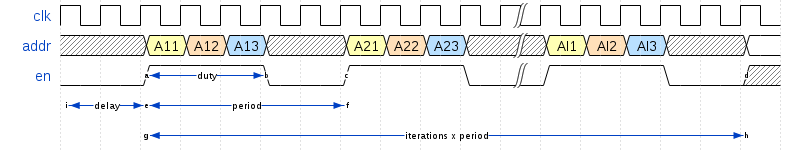
\includegraphics[height=40mm, width=155mm]{Figures/scheme_memory_properties.png}
  \caption[Representação dos parâmetros de configuração dos geradores de endereços.]{Representação dos parâmetros de configuração dos geradores de endereços.}  
  \label{fig:Representacao_gerador_enderecos}
\end{figure}

Na figura~\ref{fig:Representacao_gerador_enderecos} estão representados alguns dos parâmetros dos geradores de endereços, assim como a relação que estes têm entre si.
O entendimento correcto destes parâmetros é importante, na medida que possibilita a automatização de algumas operações complexas, exigindo um maior trabalho por parte do programador.
Refere-se que no compilador mantém-se a possibilidade de programar manualmente os geradores de endereços. Entretanto, oferece-se também a possibilidade do programador 
utilizar expressões de memória. Estas traduzidas para as respectivas configurações e, posteriormente, para {\it assembly}. 

A utilização de instruções de automatização implica uma perda de eficiência a nível do {\it assembly}. Todavia, havendo dispobilidade do programador perder alguns ciclos de relógio, que facilitem-lhe a tarefa de programar, é indicado fazê-lo. 
Nesta secção fala-se apenas das instruções de configuração manuais, devendo-se referir na secção~\ref{section:expressoes de memoria} serão analisadas as instruções automáticas.
O significado dos parâmetros está explicitado na tabela~\ref{tab:MemParameter}.


\begin{table}[h!]
    \caption[Métodos respectivos à configuração dos portos das memórias.]{Métodos respectivos à configuração dos portos das memórias.}
  \begin{center}
    \begin{tabular}{|l|L{10cm}|}
      \hline
       {\bf Parâmetro} & {\bf Descrição} \\
      \hline \hline
     % \multirow{10}{*}{Wishbone} & wb\_clk\_i & input & Clock, Recebido pelo Wishbone. \\
      \cline{1-2}
      Start(expression) & Indica a partir de que endereço de memória se começa a ler. Quando não se configura nada, o valor por omissão a nível de {\it hardware} é zero. \\
      \cline{1-2}
       Duty(expression) & Representa o número de sinais de relógio que o {\it enable} está a '1'. Quando o {\it enable} está a '1' os endereços estão a ser lidos e estão a aparecer à saída. \\
      \cline{1-2}
      Incr(expression) & É o salto de posições de memória que o gerador de endereços faz. Por exemplo, quando o incremento é 2, as posições de memória são lidas de dois em dois. \\
      \cline{1-2}
       Iter(expression) & São o número de iterações que o gerador de endereços faz até estar concluído. No registo de estado só indica que um porto de memória está pronto depois
das iterações acabarem. \\
       \cline{1-2}
      Per(expression) & É a diferença de sinais de relógio entre cada {\it enable} do gerador de endereços. O período é usado para fazer {\it loops} interiores ao equivalente de um ciclo {\it for} encadeado em C. \\
      \cline{1-2}
       Shift(expression) & Coloca o valor do {\it shift} na memória. \\
       \cline{1-2}
      Delay(expression) & É o número de ciclos de relógio que os geradores de endereços esperam antes de começarem a trabalhar.  \\
      \cline{1-2}
      Reverse(expression) & É o espelhamento dos endereços de memória. Em certas aplicações como por exemplo, a FFT, é necessário fazer espelhamento das posições de
memória para aplicar o algoritmo. \\
     
      \hline
    \end{tabular}
  \end{center}
  \label{tab:MemParameter}
\end{table}


%O {\it start} indica a partir de que endereço de memória se começa a ler, se {\it start} = 2, então a primeira posição de memória a ser lida é a posição 2.
%Quando não se configura nada, o valor por omissão a nível de {\it hardware} é zero, como o próprio {\it hardware} já tem um valor de omissão, não é necessário acrescentar mais {\it assembly} no código.

%O {\it duty} é o número de sinais de relógio que o {\it enable} está a '1'. Quando o {\it enable} está a '1' os endereços estão a ser lidos e estão a aparecer à saída.

%O período é a diferença de sinais de relógio entre cada {\it enable} do gerador de endereços. O período é usado para fazer {\it loops} interiores ao equivalente de um ciclo {\it for} encadeado em C.

%O {\it delay} é o número de ciclos de relógio que os geradores de endereços esperam antes de começarem a trabalhar. Quando se tem um circuito ligado no Versat, é preciso ter em conta que as unidades não podem começar todas ao mesmo tempo, senão perdem o sincronismo.

%O incremento é o salto de posições de memória que o gerador de endereços faz. Por exemplo, quando o incremento é 2, as posições de memória são lidas de dois em dois.

%As iterações são o número de iterações que o gerador de endereços faz até estar concluído. No registo de estado só indica que um porto de memória está pronto depois
%das iterações acabarem.

%O {\it reverse} é o espelhamento dos endereços de memória. Em certas aplicações como por exemplo, a FFT, é necessário fazer espelhamento das posições de
%memória para aplicar o algoritmo. Os dados que vão estar à saída são do endereço de memória do endereço espelhado do gerador de endereços. 


As instruções de configuração dos geradores de endereços são dadas por:

\begin{lstlisting}
		mem0.portA.setDuty(RB);
		mem0.portA.setPer(RB);
		mem0.portA.setIncr(1);
		mem0.portB.setIter(R6-1);
\end{lstlisting}

Como os portos são tratados como objectos, é necessário indicar a unidade funcional. No caso de ser uma memória, também é necessária
a indicação do porto a ela associado.
Esta situação acontece apenas nas memórias, uma vez que os portos não têm apenas a utilidade de fazer ligações (ver secção~\ref{section:metodos memorias}.



\section{Métodos exclusivos das Alu e das AluLite }
\label{section:metodos alu}


Os métodos existentes para a configuração das Alu e das AluLite podem ser visualizados na tabela~\ref{tab:instrAlu}.



\begin{table}[h!]
    \caption[Métodos referentes à Alu e à AluLite.]{Métodos referentes à Alu e à AluLite.}
  \begin{center}
    \begin{tabular}{|l|L{5cm}|}
      \hline
       {\bf Método} & {\bf Descrição} \\
      \hline \hline
     % \multirow{10}{*}{Wishbone} & wb\_clk\_i & input & Clock, Recebido pelo Wishbone. \\
      \cline{1-2}
      setOper(oper) & Define uma operação para a Alu seleccionada. \\
      \hline
    \end{tabular}
  \end{center}
  \label{tab:instrAlu}
\end{table}


Apesar do método ser o mesmo, existem determinadas operações que a AluLite não consegue realizar, mas que a Alu realiza. 
As operações que são permitidas fazer no Versat estão representadas na tabela~\ref{tab:instrOper}.


\begin{table}[h!]
    \caption[Operações permitidas pela Alu e pela AluLite.]{Operações permitidas pela Alu e pela AluLite.}
  \begin{center}
    \begin{tabular}{|l|L{8cm}|}
      \hline
       {\bf Método} & {\bf Descrição} \\
      \hline \hline
     % \multirow{10}{*}{Wishbone} & wb\_clk\_i & input & Clock, Recebido pelo Wishbone. \\
      \cline{1-2}
      + & Operação de soma. \\
      \cline{1-2}
      - & Operação de subtracção. \\
      \cline{1-2}
      \& & And lógico. \\
      \cline{1-2}
      $|$ & Or lógico. \\
      \cline{1-2}
      $\sim$\& & Nand lógico. \\
      \cline{1-2}
      $\wedge$ & Xor lógico. \\
      \cline{1-2}
      SEXT8 & Extensão de sinal de 8 bits. \\
      \cline{1-2}
      SEXT16 & Extensão de sinal de 16 bits. \\
      \cline{1-2}
      SRA & {\it Shift right} aritmético. \\
      \cline{1-2}
      SRL & {\it Shift right} lógico. \\
      \cline{1-2}
      SMPU & Comparação sem sinal. Coloca à saída o resultado da operação feita para a comparação. \\
      \cline{1-2}
      SMPS & Comparação com sinal. Coloca à saída o resultado da operação feita para a comparação. \\
      \cline{1-2}
      CLZ & Conta os bits que estão a 0 à esquerda. \\
      \cline{1-2}
      MAX & Coloca à saída o sinal de entrada mais alto. \\
      \cline{1-2}
      MIN & Coloca à saída o sinal de entrada mais baixo. \\
      \cline{1-2}
      ABS & Define uma operação para a Alu seleccionada. \\
      
     
      \hline
    \end{tabular}
  \end{center}
  \label{tab:instrOper}
\end{table}


Como as AluLites são mais limitadas, ao programa-las para uma tarefa que somente uma Alu pode realizar, surge um impedimento por parte do compilador.
As operações suportadas pela AluLite são as primeiras seis da tabela~\ref{tab:instrOper}.

A instrução
\begin{lstlisting} 
      alu0.setOper('+');      
\end{lstlisting}  
 é um exemplo de como indicar à alu0 para realizar a operação de soma. O objecto é a alu0, o método é o setOper e a operação é a soma. 


\section{Métodos exclusivos do multiplicador }
\label{section:metodos mult}

Os métodos existentes para configuração do multiplicador estão indicados na tabela~\ref{tab:instrmult}.

\begin{table}[h!]
    \caption[Métodos do multiplicador.]{Métodos do multiplicador.}
  \begin{center}
    \begin{tabular}{|l|L{9cm}|}
      \hline
      {\bf Método} & {\bf Descrição} \\
      \hline \hline
     % \multirow{10}{*}{Wishbone} & wb\_clk\_i & input & Clock, Recebido pelo Wishbone. \\
        \cline{1-2}
      setLonhi(bit) & Indica ao multiplicador se é para colocar à saída a parte baixa ou a parte alta do resultado. Recebe como argumento um bit. \\
      \cline{1-2}
       setDiv2(bit) & Indica ao multiplicador se o resultado final é para dividir por 2. Recebe como argumento um bit. \\
       
      \hline
    \end{tabular}
  \end{center}
  \label{tab:instrmult}
\end{table}




No método setLonhi, quando se envia o bit a '1', o multiplicador coloca à saída a parte mais baixa do resultado. A parte mais alta do resultado é colocada à saída quando o bit enviado é '0'. Este parâmetro é necessário, uma vez que os multiplicadores produzem resultados de 64 {\it bits}, mas apenas 32 {\it bits} podem ser postos à saída.
Quando nada é indicado, o valor é '0'.

Este processo ocorre de forma análoga no método setDiv2. Assim, quando se envia '1', o resultado é dividido por 2 e, quando se envia '0', nada acontece.
Tal como no método setLonhi, o valor por omissão é '0'.

Um exemplo do uso das instruções é:

\begin{lstlisting} 
      mult0.setLonhi('1');
      mult0.setDiv2('1');
\end{lstlisting}  




\section{Métodos exclusivos do Barrel Shifter }
\label{section:metodos bs}


Os métodos exclusivos do {\it barrel shifter} estão na tabela~\ref{tab:instrBs}.


\begin{table}[h!]
    \caption[Métodos exclusivos do {\it barrel shifter}.]{Métodos exclusivos do {\it barrel shifter}.}
  \begin{center}
    \begin{tabular}{|l|L{5cm}|}
      \hline
      {\bf Método} & {\bf Descrição} \\
      \hline \hline
     % \multirow{10}{*}{Wishbone} & wb\_clk\_i & input & Clock, Recebido pelo Wishbone. \\
      \cline{1-2}
      setLNA(oper) & \textcolor{red}{Meter aqui a descrição} \\
      \cline{1-2}
      setLNR(oper) & \textcolor{red}{Meter aqui a descrição} \\
      \cline{1-2}
      
      \hline
    \end{tabular}
  \end{center}
  \label{tab:instrBs}
\end{table}



\section{Métodos de conexão }
\label{section:metodos connect}

Nesta secção podem ser encontrados os métodos de conexão entre as unidades funcionais. Estes estão explicitados na tabela~\ref{tab:instrconnect}.

\begin{table}[h!]
    \caption[Métodos respectivos à memória.]{Métodos respectivos à memória.}
  \begin{center}
    \begin{tabular}{|l|L{7cm}|}
      \hline
      {\bf Método} & {\bf Descrição} \\
      \hline \hline
     % \multirow{10}{*}{Wishbone} & wb\_clk\_i & input & Clock, Recebido pelo Wishbone. \\
     
      \cline{1-2}
      connectPortA(FU) & Conecta o porto A de uma unidade funcional à saída da unidade funcional passada como argumento. \\
      \cline{1-2}
      connectPortA(mem, port) & Conecta o porto A da unidade funcional à saída de uma memória passada como argumento. Quando se conecta a uma memória é encessário indicar o porto. \\
      \cline{1-2}
      connectPortB(FU) & Conecta o porto B da unidade funcional à saída da unidade funcional passada como argumento. \\
      \cline{1-2}
       connectPortB(mem, port) & Conecta o porto B da unidade funcional à saída da unidade funcional passada como argumento. Quando se conecta a uma memória é encessário indicar o porto. \\
      \cline{1-2}
      connect(FU) & Conecta um porto de memória a uma unidade funcional diferente de outra memória. Recebe como argumento a respectiva unidade funcional. \\
       \cline{1-2}
      connect(mem, port) & Conecta um porto de memória a uma memória. Recebe como argumento a memória e o porto ao qual se quer conectar.\\

      \hline
    \end{tabular}
  \end{center}
  \label{tab:instrconnect}
\end{table}

Os métodos connect são aplicados apenas em memórias, enquanto os demais são utilizados para as restantes unidades funcionais. Os métodos de conexão
das memórias são diferentes dos métodos das restantes unidades funcionais, uma vez que os portos das memórias são tratados como objectos, como já referido anteriormente.

Um exemplo do uso das instruções é:

\begin{lstlisting} 
 
 mem0.portA.connect(mem2, 'a');
 mem0.portB.connect(alu0);
 alu0.connectPortA(mult1);
 mult3.connectPortB(mem2, 'a');	
 
\end{lstlisting}

\section{Métodos para desactivar unidades funcionais }
\label{section:metodos disable}

Os métodos para desactivar unidades funcionais encontram-se na tabela~\ref{tab:instrDisable}.



\begin{table}[h!]
    \caption[Métodos para desactivar unidades funcionais.]{Métodos para desactivar unidades funcionais.}
  \begin{center}
    \begin{tabular}{|l|L{5cm}|}
      \hline
       {\bf Método} & {\bf Descrição} \\
      \hline \hline
     % \multirow{10}{*}{Wishbone} & wb\_clk\_i & input & Clock, Recebido pelo Wishbone. \\
      \cline{1-2}
      disableFU() & Desactiva a unidade funcional à qual o objecto está associado. \\
      \hline
    \end{tabular}
  \end{center}
  \label{tab:instrDisable}
\end{table}


Esta instrução é utilizada quando se quer trabalhar a unidade funcional como um registo. É impossível desactivar memórias.
Um exemplo do uso é:

\begin{lstlisting}
 mult0.disableFU();
\end{lstlisting}


\section{Expressões de registos}
\label{section:expressoes registos}


A linguagem C++ do Versat suporta expressões com muitos registos, que podem ter uma dimensão muito grande, desde que existam recursos. Como 
não existe uma pilha de memória, é impossível declarar variáveis. O registo RB é utilizado como auxiliar no cálculo de expressões grandes, sendo necessário ter
cuidado com o seu uso para guardar dados, uma vez que podem ser apagados em certa altura. Não é necessário declarar os registos.

Devido ao {\it assembly} limitado do controlador, nem todas as operações são permitidas. As operações permitidas estão disponíveis na tabela~\ref{tab:instrControlador}.

\begin{table}[h!]
    \caption[Operações suportadas pelas expressões de registos.]{Operações suportadas pelas expressões de registos.}
  \begin{center}
    \begin{tabular}{|l|L{5cm}|}
      \hline
       {\bf Método} & {\bf Descrição} \\
      \hline \hline
     % \multirow{10}{*}{Wishbone} & wb\_clk\_i & input & Clock, Recebido pelo Wishbone. \\
      \cline{1-2}
      + & Soma. \\
       \cline{1-2}
      - & Substracção. \\
       \cline{1-2}
      \& & And lógico. \\
       \cline{1-2}
      $>>$ & {\it Shift right}. \\
       \cline{1-2}
      $<<$ & {\it Shift left}. \\
      \hline
    \end{tabular}
  \end{center}
  \label{tab:instrControlador}
\end{table}

Também é suportado o uso de parêntesis e são respeitadas as ordens aritméticas - estas consistem primeiro no cálculo das operações matemáticas entre parêntesis, seguido dos deslocamentos e ands lógicos, finalizando com as operações de soma e subtracção).

\textcolor{red}{Tirar do flex o suporte para a divisão.}

Um exemplo do uso de expressões é dado por:

\begin{lstlisting}
 
 R1 = R2+R3+R4-R5&R6+R7-R8;
 
\end{lstlisting}

\section{If condicional}
\label{section:if condicional}

O compilador de C++ do Versat suporta instruções condicionais, assim como condicionais encadeadas. Um exemplo do uso da condição if é:

\begin{lstlisting}
 if(R1+R3!=0) {
	R5=2;  }
\end{lstlisting}

A condição suporta apenas expressões com dois operandos. Exceptuando esta limitação, a condição é utilizada de forma análoga a C++ regular.

\section{Else condicional}
\label{section:else condicional}


O uso da condição {\it else} é feito de forma idêntica a C++ regular. Um exemplo da aplicação da condição {\it else} é:

\begin{lstlisting}
 
 if(R5!=0) {
      if(R6!=0)  R6=1;
      else R6=2; }
      
else {
    R5=2; }
 
\end{lstlisting}

\section{Ciclo while}
\label{section:ciclo while}

Tal como nas condições, os ciclos são usados da mesma maneira que em C++ regular. A limitação de suportar apenas expressões com dois operandos mantém-se.

Um exemplo de aplicação do ciclo {\it while} é:

\begin{lstlisting}
int main() {
    R5=1000;
    while(R5<=40) { 
	    R5=6+R5;
	    R7=R7+R4+2;  }
  return 0;  }
\end{lstlisting}


\section{Ciclo for}
\label{section:ciclo for}

Os ciclos {\it for} são iguais ao C++ regular. No local do incremento, as instruções Rx++, Rx- -, ++Rx e - -Rx não são suportadas.

Um exemplo de aplicação do ciclo {\it for} é:

\begin{lstlisting}
 int main()  {
      for(R4=0;R4<20;R4=R4+1) {
	      for(R5=0;R5<5;R5=R5+1)  {
		    R6=R7+R8+R6;  }
		    
	      R7=R7+R4;  }
 
 return 0; }
\end{lstlisting}


\section{Ciclo do while}
\label{section:ciclo do while}

Tal como as outras instruções de ciclo, os ciclos {\it do while} são iguais ao C++ regular. Um exemplo de aplicação do ciclo {\it do while} é:

\begin{lstlisting}
 
 int main() {
      do {
	  do  {
	      R1=R1+2+R5; }
	  while(R1!=20);
	  R5=R5+1;  }
      while(R5<50);
 
 return 0; }
 
\end{lstlisting}



\section{Salto goto}
\label{section:salto goto}


Existem etiquetas que não se podem utilizar na instrução {\it goto}. Assim, o compilador aplica etiquetas internas para implementar as instruções de {\it if}, {\it while}, {\it for}, {\it do while} e {\it wait}. 
Estas etiquetas podem ser encontradas na tabela~\ref{tab:labels}.




\textcolor{red}{ainda não está a dar erro quando as etiquetas não são permitidas}

Um exemplo do uso da instrução {\it goto} é:

\begin{lstlisting}
 
 begin	R4=3;

 goto(begin);
 
\end{lstlisting}

Esta instrução em C++ regular raramente é usada, mas no C++ do Versat é extremamente útil na programação de pseudo-rotinas.

\begin{table}[h!]
    \caption[Etiquetas que o utilizador não pode usar.]{Etiquetas que o utilizador não pode usar.}
  \begin{center}
    \begin{tabular}{|l|l|}
      \hline
       Etiqueta & Instrução relacionada  \\
      \hline \hline
     % \multirow{10}{*}{Wishbone} & wb\_clk\_i & input & Clock, Recebido pelo Wishbone. \\
      \cline{1-2}
      ifStatment  & if  \\
      \cline{1-2}
       whileStatment & while \\
       \cline{1-2}
       whileDirectStatment & while  \\
       \cline{1-2}
       forDirectStatment & for \\
       \cline{1-2}
       forStatment & for  \\
       \cline{1-2}
       elseStatment & else \\
       \cline{1-2}
       waitres & wait  \\
      
      \hline
    \end{tabular}
  \end{center}
  \label{tab:labels}
\end{table}


\section{Expressões de memória}
\label{section:expressoes de memoria}


O compilador do Versat também permite expressões de memória, sendo o seu algoritmo dado por:

\begin{lstlisting}

for(i=0;i<iter;i++) {
  for(j=0;j<per;j++)  
  memxX[start+j(per+shift)+incr*i] = memxX[start+j(per+shift)+incr*i];  }

\end{lstlisting}

O período e o número de iterações é comum a todas as memórias utilizadas nas expressões. Os outros parâmetros variam consoante a memória em causa.
Os multiplicadores e alus necessários para efectuar as operações entre memórias são definidas automaticamente. Assim, não é preciso indicar as alus e os 
multiplicadores a aplica, uma vez que isto é feito internamente.

\textcolor{red}{Fazer a libertação automática do hardware!!!!!!!!}


As variáveis i e j são fixas, não sendo necessária uma declaração prévia. 


Um exemplo da aplicação das expressões de memória é:

\begin{lstlisting}
for(i=0;i<1023;i++) {
	mem0A[j(1)+1*i]=mem2A[j(1)+2*i]+mem2B[1024+j(1)+1*i];  
	mem0B[1024+j(1)+1*i]=mem3B[1024+j(1)+1*i]; 
	mem1A[j(1)+1*i]=mem3A[j(1)+2*i]; }
\end{lstlisting}


Quando o {\it for} interior não existe, o valor do período por omissão é '1'.



\section{Return}
\label{section:return}


A instrução de {\it return} é o final da função {\it main} em C++ do Versat. Após {\it return} é possível escrever código, porém este é acessível apenas 
pela instrução {\it goto} (explicada na secção~\ref{section:salto goto}). 
Um exemplo da utilização do {\it return} é:

\textcolor{red}{Meter um goto boot ROM no código para quando estes problemas acontecerem o Versat não continuar a correr. Meter um exemplo do return com codigo por baixo deste!!!!!!!}


\begin{lstlisting}
 
 int main() {
 
    return 0;  }
 
\end{lstlisting}



\section{Asm}
\label{section:return}

A instrução asm é aplicada para permitir a escrita de {\it assembly} em código C++ do Versat. O asm varia consoante o compilador. No presente caso, optou-se
por uma utilização análoga a do g++. Um exemplo do uso da instrução asm é:

\begin{lstlisting}
 
 int main() {
 
 asm {
      ldi ALU_ADD
	wrc ALU0_CONFIG_ADDR,ALU_CONF_FNS_OFFSET
	ldi smul1
	wrc ALU0_CONFIG_ADDR,ALU_CONF_SELA_OFFSET
	ldi salu0
	wrc ALU0_CONFIG_ADDR,ALU_CONF_SELB_OFFSET
	ldi 1    }
	
	return 0;
 
 }
 
\end{lstlisting}

\section{Comentários}
\label{chapter:comentarios}

Os comentários em C++ do Versat são exactamente iguais ao C++ regular. Um exemplo da utilização de comentários em C++ do Versat é dado em:

\begin{lstlisting}
 // R4=0;
 /*if(R5==0) {
      R2=R3+R4;  }  */
\end{lstlisting}



\chapter{Exemplos de código}
\label{chapter:exemplos de codigo}


\section{Adição de vectores}
\label{section:vec_add}


\section{Produto interno complexo}
\label{section:complex_dot_product}


\section{FFT}
\label{section:FFT}

\textcolor{red}{meter o codigo fft\_expressions.cpp}

\cleardoublepage

